% chktex-file 8
\chapter{Resultados}

\section{Datos analizados}

La evaluación principal se toma de la configuración estable del 18 de junio de 2026. El entrenamiento \texttt{train\_2026-06-18\_11-21} contiene 548 generaciones completas en \texttt{Training\_Summary.csv} y 16432 registros en \texttt{Fitness\_Debug.csv}. La columna \texttt{N} declara 16440 vehículos, por lo que la cobertura del fichero de detalle es del 99.95\%. El informe automático no detecta alertas fuertes de desalineación, pero esta diferencia de ocho filas se conserva como limitación del conjunto.

La evaluación de test agrega las cuatro carpetas del 18 de junio: \texttt{12-41}, \texttt{14-03}, \texttt{14-39} y \texttt{14-51}. En conjunto reúnen 21 ejecuciones completas y 1134 vehículos, con 21 observaciones para cada uno de los 54 puntos de aparición. Los cuatro informes presentan cobertura del 100\%, no descartan filas y clasifican todos los registros como test. La hora identifica cada carpeta archivada; no se interpreta como una variable experimental.

Los tamaños efectivos se obtienen de los CSV\@: 30 vehículos por generación de entrenamiento y 54 por ejecución de test. Esta comprobación es necesaria porque \texttt{PopulationSize} es editable en la instancia del mapa y su valor por defecto no describe necesariamente la sesión archivada. También se detectó que las carpetas de test \texttt{2026-06-11\_11-55} y \texttt{2026-06-11\_13-08} contienen un \texttt{Fitness\_Debug.csv} idéntico; en las comparaciones se cuenta una sola vez. La Tabla~\ref{tab:configuracion-experimental} fija la configuración experimental del bloque de referencia utilizado en el resto del capítulo.

\begin{table}[H]
\centering
\caption{Configuración experimental documentada del bloque de referencia.}%
\label{tab:configuracion-experimental}
\begin{tabularx}{0.96\textwidth}{L{3.6cm}X}
\toprule
\textbf{Elemento} & \textbf{Configuración usada en la lectura de resultados}\\
\midrule
Entrenamiento de referencia & \texttt{train\_2026-06-18\_11-21}, 548 generaciones completas, 30 vehículos efectivos por generación y 30 puntos de aparición únicos en los CSV.\\
Test agregado & Cuatro sesiones del 18 de junio, 21 ejecuciones completas, 54 puntos de aparición y 1134 evaluaciones.\\
Modelo en test & Pesos cargados sin mutación durante la evaluación; el test mide comportamiento de un modelo fijo, no aprendizaje en línea.\\
Criterio de acierto & Causa terminal no incluida entre fallos y al menos 60 segundos de vida. \texttt{TestMinFitness} figura como 25000, pero \texttt{TestUseFitness} está desactivado para este criterio.\\
Aleatoriedad & No consta una semilla global documentada para reproducir bit a bit mutaciones o elecciones de trayectoria; la trazabilidad se conserva mediante carpetas, modelos, CSV e informes.\\
Duración de episodio & En \texttt{FITNESS 18-06-2026}, \texttt{MaxTimeAlived} es 100 para test y el límite de entrenamiento es 120 segundos; el análisis usa tiempo de vida y causa terminal, no solo supervivencia.\\
Mutación registrada & El test se ejecuta sin mutación. En entrenamiento, los CSV documentan por individuo el número de pesos modificados y la magnitud media; en el bloque de referencia se observan 11.95 pesos modificados de media y un máximo de 38 por individuo.\\
\bottomrule
\end{tabularx}
\caption*{\textit{\textbf{Fuente.} Elaboración propia a partir de \texttt{EVOLUTIONMANAGER}, \texttt{FITNESS}, CSV e informes del 18 de junio.}}
\end{table}

\Needspace{8\baselineskip}
Los bloques posteriores de final de junio y comienzo de julio se emplean como pruebas de regresión y diagnóstico, no como nueva referencia principal. En esa serie aparecen recuperaciones parciales, caídas por \texttt{STOP\_VIOLATION}, sesiones demasiado cortas y nuevos indicadores sobre cedas, solapes y bloqueo en cruces. El 2 de julio alcanza 193 aciertos sobre 354 evaluaciones, un 54.52\%, pero procede de un único bloque más pequeño que la referencia del día 18. El 3 de julio cambia además el modo experimental: se activa \texttt{FreeRun}, con coches vivos censurados y respawn por spawnpoint. Se revisan dos sesiones de ese tipo, una dominada por \texttt{LAZY} y otra por \texttt{NAV\_VIOLATION}; ambas deben interpretarse como simulación libre de tráfico y no como test estadístico generacional. Por ello, los resultados principales del capítulo se apoyan en la configuración de referencia evaluada el 18 de junio y las sesiones posteriores se interpretan como evidencia para decidir las siguientes correcciones.

Tras incorporar las carpetas nuevas de julio se revisaron también los entrenamientos \texttt{train\_2026-07-06\_02-22} y \texttt{train\_2026-07-06\_11-47}, el diagnóstico \texttt{FreeRun} del 6 de julio y cinco bloques de test del 7 de julio. El bloque \texttt{test\_2026-07-07\_16-45}, con 50 generaciones y 2950 evaluaciones declaradas, se analiza de forma separada en la Sección~\ref{sec:validacion-posterior}. Su interés es comprobar la versión final instrumentada del programa, no reescribir automáticamente la referencia histórica del 18 de junio.

\section{Resumen cuantitativo}

\begin{table}[htbp]
\centering
\caption{Resultados principales del entrenamiento y del bloque de test del 18 de junio de 2026.}%
\label{tab:resultados-principales}
\begin{tabular}{lrr}
\toprule
\textbf{Métrica} & \textbf{Entrenamiento} & \textbf{Test agregado}\\
\midrule
Generaciones o ejecuciones & 548 & 21\\
Registros de vehículos & 16432 & 1134\\
\textit{BestFit} máximo & 134959.45 & 80104.07\\
\textit{MeanFit} medio & 30049.20 & 44619.47\\
\textit{MeanFit} mediano & 29922.54 & 45313.89\\
Tiempo medio de vida & 74.98 s & 77.91 s\\
Ejecuciones con \textit{MeanFit} negativo & 0.00\% & 0.00\%\\
Colisiones & 45.54\% & 40.04\%\\
Fallos legales & 2.12\% & 2.29\%\\
\texttt{LAZY} & 0.00\% & 0.00\%\\
Tasa de acierto operativo & \multicolumn{1}{c}{No aplica} & 57.50\%\\
\bottomrule
\end{tabular}
\caption*{\textit{\textbf{Fuente.} Elaboración propia a partir de los CSV del proyecto.}}
\end{table}

El test no mejora el modelo durante la ejecución: carga pesos fijos y desactiva la mutación. Su mayor \textit{MeanFit} responde a que cambia la distribución de puntos y trayectorias y a que cada ejecución cubre los 54 spawns de test. Por ello, la tabla~\ref{tab:resultados-principales} describe cada modo, pero no permite atribuir la diferencia de fitness únicamente a la calidad de la política.

\clearpage
\section{Evolución del entrenamiento}

El mejor fitness se alcanza en la generación 56, con 134959.45, y el fitness medio máximo en la generación 33, con 44373.00. Ninguna de las 548 generaciones presenta \textit{MeanFit} negativo.

\begin{figure}[H]
\centering
\caption[Tendencia del fitness en el entrenamiento del 18 de junio de 2026.]{Tendencia del fitness en el entrenamiento del 18 de junio de 2026. La gráfica combina valores por generación con medias móviles de 30 generaciones generadas por el script de análisis.}%
\label{fig:tendencia-entrenamiento}
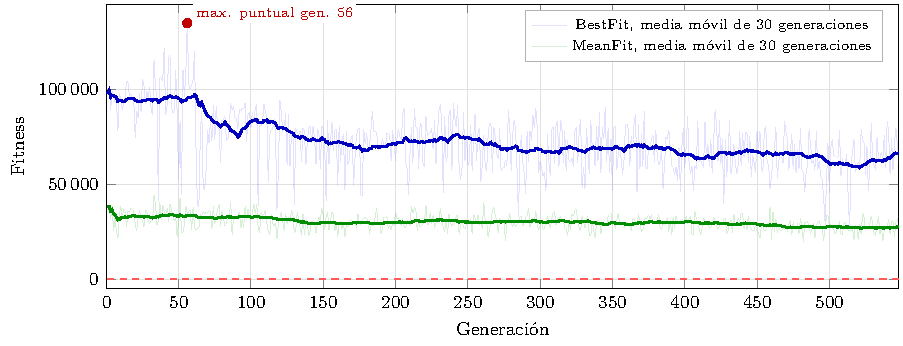
\includegraphics[width=0.92\textwidth]{assets/tendencia_entrenamiento_2026-06-18.pdf}
\caption*{\textit{\textbf{Fuente.} Análisis generado a partir de \texttt{Training\_Summary.csv}.}}
\end{figure}

La figura~\ref{fig:tendencia-entrenamiento} muestra variabilidad persistente y obliga a separar supervivencia de aptitud. Entre las primeras y las últimas 50 generaciones, el \textit{MeanFit} desciende un 17.5\%, de 33263.23 a 27433.45, mientras el tiempo medio aumenta un 43.1\%, de 54.83 a 78.46 segundos. El informe no identifica convergencia clara y registra 492 generaciones desde el último máximo. El modelo aprende a permanecer activo durante más tiempo, pero esa supervivencia no se traduce en una mejora monotónica del objetivo; por tanto, el entrenamiento debería interpretarse como una búsqueda todavía abierta, no como una convergencia cerrada.

La tabla~\ref{tab:evolucion-red-fitness} sitúa este resultado dentro de la evolución técnica de la red y del fitness durante el proyecto.

\begin{table}[H]
\centering
\caption{Evolución de la red neuronal y del fitness durante el proyecto.}%
\label{tab:evolucion-red-fitness}
\begin{tabularx}{0.96\textwidth}{L{2.5cm}L{3.6cm}X}
\toprule
\textbf{Periodo} & \textbf{Arquitectura y entradas} & \textbf{Evolución del fitness}\\
\midrule
Enero & 11 sensores, velocidad, velocidad angular y bias; 12 neuronas ocultas. & Función centrada en avance, centrado lateral, giro y castigos simples por marcha atrás, colisión o estancamiento. Adecuada para la línea de pruebas inicial, insuficiente para ciudad completa.\\
Febrero-marzo & Sensores en abanico y primeros bordes de intersección filtrados por trayectoria. & El fitness deja de premiar solo avance y empieza a distinguir velocidad segura, corrección lateral, retroceso y estancamiento. El cambio a múltiples spawns obliga a normalizar por zona.\\
Abril & Vector ampliado con contexto de tráfico, distancia a línea de parada y codificación one-hot; transición hacia 20 entradas. & El fitness incorpora semáforos, stops, cedas, espera legal, marcha atrás, suavizado y telemetría ampliada. Aparecen regresiones que ya pueden explicarse con CSV.\\
Mayo-junio & Capa oculta consolidada en 16 neuronas; 320 pesos \texttt{IH} y 32 pesos \texttt{HO}. & Se estabilizan persistencia, mutación dinámica, normalización por spawn y métricas de rotonda. El 18 de junio se obtiene la referencia principal de test.\\
Junio-julio & Misma red, pero con percepción de otros coches, distancia efectiva y modo libre. & El fitness añade solapes, penalización real de distancia de seguridad, colas de ceda, bloqueo en cruce y diagnóstico de coches físicos no fantasma.\\
\bottomrule
\end{tabularx}
\caption*{\textit{\textbf{Fuente.} Elaboración propia a partir de descripciones fechadas de \texttt{REDNEURONAL}, \texttt{FITNESS} y \texttt{EVOLUTIONMANAGER}.}}
\end{table}

De los 16432 registros, 8511 terminan por tiempo y 7483 por colisión. Los 348 fallos legales representan el 2.12\%, y no aparece ninguna muerte \texttt{LAZY}. Los 90 casos restantes corresponden a 54 \texttt{FLIPPED} y 36 \texttt{REVERSE}, por lo que no quedan razones terminales sin clasificar en el desglose principal. El analizador marca 1985 posibles atascos ante stop y 1011 ante ceda dentro de las finalizaciones por tiempo. Son candidatos heurísticos, no infracciones confirmadas, pero explican por qué el tiempo de vida no puede utilizarse como único indicador.

La sesión registra además 5365 entradas en rotonda, 1075 completaciones confirmadas por una nueva entrada y 2350 colisiones dentro de ese contexto. La tasa de completado del 20.04\% es un límite inferior porque el contador solo confirma la maniobra al alcanzar de nuevo el trigger de entrada. El saldo específico de rotonda es negativo, con \(-553966{.}78\) puntos acumulados, debido principalmente a la penalización de aceleración.

\Needspace{10\baselineskip}
\section{Evaluación de test}

El criterio implementado considera fallo cualquier colisión, infracción, estancamiento, corrección o marcha atrás incorrecta, vuelco, red inválida o navegación fuera de zona; también exige al menos 60 segundos de vida. El umbral de fitness de 25000 está configurado, pero desactivado mediante \texttt{TestUseFitness}. En esta memoria se denomina acierto operativo a una evaluación que supera ese criterio de test: no termina por una causa de fallo y alcanza el tiempo mínimo exigido. No equivale a una validación clínica ni garantiza que el vehículo resuelva todos los escenarios urbanos de forma robusta. Con estas reglas, el bloque del 18 de junio obtiene 652 aciertos de 1134 evaluaciones, un 57.50\%. El intervalo de confianza de Wilson al 95\% se sitúa entre el 54.60\% y el 60.34\%~\cite{wilson}. Este intervalo cuantifica la incertidumbre de una proporción binomial dentro del bloque agregado; no mide la variabilidad entre entrenamientos independientes ni sustituye a una repetición completa con semillas controladas. Las cuatro sesiones oscilan entre el 53.70\% y el 61.42\%, con una mediana del 57.04\%.

Para evitar una interpretación excesiva de esa cifra, la tabla~\ref{tab:limitaciones-experimentales} resume las principales restricciones del bloque de referencia. Todas ellas se mantienen en la lectura de conclusiones y líneas futuras.

\begin{table}[H]
\centering
\caption{Limitaciones de interpretación del bloque de referencia.}%
\label{tab:limitaciones-experimentales}
\begin{tabularx}{0.96\textwidth}{L{3.25cm}X}
\toprule
\textbf{Aspecto} & \textbf{Limitación}\\
\midrule
Alcance del acierto & El 57.50\% mide acierto operativo bajo el criterio de test configurado; no valida uso clínico ni conducción autónoma robusta.\\
Mapa y cobertura & Las 1134 evaluaciones cubren 54 puntos de aparición del mapa actual, pero no prueban generalización a otros escenarios urbanos.\\
Aleatoriedad & No consta en las fuentes revisadas una semilla aleatoria global fijada para reproducir bit a bit mutaciones o elecciones de salida. La trazabilidad se apoya en modelos, CSV y carpetas archivadas.\\
Convergencia & El entrenamiento del 18 de junio no muestra convergencia clara: mejora la supervivencia, pero el fitness medio desciende entre el inicio y el final.\\
Regresiones posteriores & Las pruebas de final de junio y julio introducen cambios de fitness, señalización y tráfico; sirven como diagnóstico, no como sustitución automática de la referencia.\\
Línea base externa & No se compara contra un controlador reglado, una política supervisada ni otro simulador; las mejoras se interpretan respecto a bloques previos del propio proyecto.\\
\bottomrule
\end{tabularx}
\caption*{\textit{\textbf{Fuente.} Elaboración propia a partir de los CSV, informes de análisis y descripciones fechadas del proyecto.}}
\end{table}

La tabla~\ref{tab:comparacion-bloques-test} resume la secuencia de pruebas archivadas. No constituye un experimento controlado entre fechas, porque durante junio cambian el fitness, las intersecciones, el número de spawns y los modelos. Se utiliza para mostrar la evolución observada, no para atribuir causalidad a una modificación aislada. En esta tabla, el fitness medio se calcula directamente sobre \texttt{Fitness\_Final}; por ello puede diferir ligeramente del promedio de \textit{MeanFit} de la tabla~\ref{tab:resultados-principales}. El duplicado exacto del 11 de junio se excluye. Cuando el resumen declara más evaluaciones que registros completos de detalle, se conserva la cifra de detalle para el fitness y la vida media, y la tasa de acierto procede de \texttt{Test\_Summary.csv}.

\Needspace{20\baselineskip}
{\small
\setlength{\tabcolsep}{4pt}
\begin{longtable}{L{2.6cm}rrrr}
\caption{Evolución de los bloques de test archivados entre junio y julio de 2026.}\label{tab:comparacion-bloques-test}\\
\toprule
\textbf{Fecha} & \textbf{Evaluaciones} & \textbf{Acierto} & \textbf{Fitness medio} & \textbf{Vida media}\\
\midrule
\endfirsthead%
\caption[]{Evolución de los bloques de test archivados entre junio y julio de 2026 (continuación).}\\
\toprule
\textbf{Fecha} & \textbf{Evaluaciones} & \textbf{Acierto} & \textbf{Fitness medio} & \textbf{Vida media}\\
\midrule
\endhead%
\bottomrule
\multicolumn{5}{>{\centering\arraybackslash}p{0.92\textwidth}}{\textit{\textbf{Fuente.} Elaboración propia a partir de \texttt{Fitness\_Debug.csv} y \texttt{Test\_Summary.csv}.}}\\
\endfoot%
\bottomrule
\multicolumn{5}{>{\centering\arraybackslash}p{0.92\textwidth}}{\textit{\textbf{Fuente.} Elaboración propia a partir de \texttt{Fitness\_Debug.csv} y \texttt{Test\_Summary.csv}.}}\\
\endlastfoot%
2 de junio & 1975 & 16.51\% & 27195.46 & 46.16 s\\
5 de junio & 2080 & 18.51\% & 26599.02 & 44.98 s\\
8 de junio & 1560 & 25.19\% & 31295.04 & 53.13 s\\
11 de junio & 1092 & 29.67\% & 33200.70 & 52.90 s\\
15 de junio & 431 & 28.01\% & 32758.50 & 53.90 s\\
16 de junio & 1890 & 26.51\% & 34104.90 & 55.10 s\\
17 de junio & 540 & 39.63\% & 40305.20 & 67.50 s\\
18 de junio & 1134 & 57.50\% & 44631.86 & 77.91 s\\
22 de junio & 550 & 52.91\% & 44296.62 & 76.20 s\\
23 de junio & 1094 & 16.27\% & 28264.74 & 50.21 s\\
26 de junio & 467 & 49.89\% & 41869.89 & 73.34 s\\
29 de junio & 1179 & 30.42\% & 33191.28 & 61.07 s\\
30 de junio & 236 & 46.61\% & 32663.97 & 75.06 s\\
1 de julio & 767 & 27.38\% & 17578.78 & 56.23 s\\
2 de julio & 354 & 54.52\% & 30276.78 & 80.27 s\\
\end{longtable}
}

Frente al 8 de junio, el bloque del día 18 sube 32.31 puntos de acierto operativo, un 42.6\% el fitness final medio y un 46.6\% la vida media. Como la serie cae el día 15 y en varias sesiones del 16, las mejoras se aceptan solo tras repeticiones.

Los bloques posteriores muestran por qué no basta con seguir la fecha más reciente. La serie pasa por una fase próxima a la referencia, una degradación normativa fuerte, una recuperación desigual y una mejora parcial en los dos tests del 30 de junio. Este último bloque reúne solo 236 evaluaciones válidas, por lo que no tiene el peso estadístico del día 18, pero sí confirma que el comportamiento debe valorarse por familias de fallo y no por una única cifra agregada. Ese contraste convierte las sesiones posteriores en material de diagnóstico, no en sustitución directa del bloque de referencia.

\newpage
\section{Razones de finalización}

Las 652 finalizaciones por tiempo coinciden con los aciertos declarados en el resumen de test. Entre los 482 fallos hay 454 colisiones, 23 infracciones de stop, tres infracciones de tráfico y dos casos de marcha atrás. No aparecen \texttt{LAZY}, \texttt{YIELD\_VIOLATION}, \texttt{NAV\_VIOLATION} ni \texttt{INVALID\_BRAIN}. La Tabla~\ref{tab:codigos-terminales} resume cómo se interpretan estos códigos y los subtipos introducidos en iteraciones posteriores. La Figura~\ref{fig:distribucion-test} visualiza esa distribución para que la lectura no dependa solo de la tabla de resultados agregados.

\begin{table}[H]
\centering
\caption{Lectura de los principales códigos terminales exportados.}%
\label{tab:codigos-terminales}
\footnotesize
\begin{tabularx}{0.98\textwidth}{L{3.6cm}X L{2.4cm}}
\toprule
\textbf{Código o familia} & \textbf{Significado operativo} & \textbf{Lectura en test}\\
\midrule
\texttt{TIMEFINISHED} & El vehículo alcanza el límite temporal del episodio sin muerte por fallo. & Acierto si supera el tiempo mínimo.\\
\texttt{COLLISION\_WITH\_*} & Colisión contra borde de intersección, volumen de navegación, vehículo u otro actor relevante. & Fallo.\\
\texttt{STOP\_VIOLATION} & Incumplimiento genérico de stop en versiones previas. & Fallo legal.\\
\texttt{STOP\_VIOLATION\_EXIT} & Salida de la zona de stop sin validación correcta. & Fallo legal.\\
\shortstack[l]{\texttt{STOP\_VIOLATION}\\\texttt{\_TIMEOUT}} & Agotamiento del tiempo de validación de stop en la lógica posterior. & Fallo legal.\\
\shortstack[l]{\texttt{YIELD\_VIOLATION}\\\texttt{\_EXIT}/\texttt{\_TIMEOUT}} & Salida indebida o espera agotada en ceda el paso. & Fallo legal.\\
\texttt{NAV\_VIOLATION} & Salida de zona válida o conflicto con la navegación instrumentada. & Fallo.\\
\texttt{LAZY} & Estancamiento sin justificación de tráfico suficiente. & Fallo.\\
\texttt{REVERSE}/\texttt{BACKWARDS} & Marcha atrás o riesgo de retroceso incorrecto. & Fallo.\\
\shortstack[l]{\texttt{FLIPPED}\\\texttt{INVALID\_BRAIN}} & Vuelco físico o red incompatible tras guardas de inferencia. & Fallo.\\
\texttt{OVERLAP\_TIMEOUT} & Solape prolongado entre vehículos en versiones con coches no fantasma. & Fallo.\\
\bottomrule
\end{tabularx}
\caption*{\textit{\textbf{Fuente.} Elaboración propia a partir de \texttt{Fitness\_Debug.csv}, \texttt{EVOLUTIONMANAGER}, \texttt{FITNESS} e \texttt{INTERSECTIONS}.}}
\end{table}

\newpage
\begin{figure}[H]
\centering
\caption[Distribución de aciertos y causas de fallo en test.]{Distribución de aciertos operativos y causas de fallo en el bloque de test del 18 de junio de 2026.}%
\label{fig:distribucion-test}
\small
\begin{tabularx}{0.94\textwidth}{L{3.2cm}rX}
\toprule
\textbf{Resultado} & \textbf{Casos} & \textbf{Proporción sobre 1134 evaluaciones}\\
\midrule
Acierto operativo & 652 & \rule{4.60cm}{0.18cm}\;57.50\%\\
Colisión & 454 & \rule{3.20cm}{0.18cm}\;40.04\%\\
\texttt{STOP\_VIOLATION} & 23 & \rule{0.16cm}{0.18cm}\;2.03\%\\
Infracción de tráfico & 3 & \rule{0.03cm}{0.18cm}\;0.26\%\\
Marcha atrás & 2 & \rule{0.02cm}{0.18cm}\;0.18\%\\
\bottomrule
\end{tabularx}
\caption*{\textit{\textbf{Fuente.} Elaboración propia a partir de \texttt{Test\_Summary.csv} y \texttt{Fitness\_Debug.csv}.}}
\end{figure}

El actor con más colisiones es \texttt{BP\_IntersectionBorder221}, con 94 casos. Le siguen \texttt{NavModifierVolume43}, con 64, y \texttt{NavModifierVolume35}, con 63. Los tres reúnen 221 fallos, el 48.7\% de todas las colisiones del bloque. La concentración mantiene como prioridad la revisión geométrica de esos elementos y de los recorridos que conducen hasta ellos.

\section{Comportamiento ante señalización}

En contexto de parada, el 99.34\% del uso acumulado de los pedales corresponde al freno y el 0.66\% al acelerador. Los registros contabilizan 622 stops y 1692 cedas completados; un mismo vehículo puede superar varias señales, por lo que estas cifras miden eventos y no coches únicos. Las 26 infracciones legales suponen el 2.29\% del bloque.

Estos datos confirman que la señalización modifica la acción del controlador, pero no demuestran por sí solos que toda espera sea correcta. La gran diferencia entre completaciones y muertes legales convive con finalizaciones por tiempo que el detector heurístico puede clasificar como atasco. En los cuatro informes del 18 de junio aparecen seis candidatos fuertes de atasco en ceda y cuatro en stop dentro de las 652 finalizaciones por tiempo, es decir, el 0.92\% y el 0.61\% de los aciertos operativos. Son señales de revisión, no fallos confirmados, pero obligan a no leer \texttt{TIMEFINISHED} como conducción útil garantizada. Para validar una señal concreta siguen siendo necesarias la progresión de ruta, la duración continua de la detención y la inspección del spawn asociado.

\section{Comportamiento en rotondas}

El bloque de test registra 443 entradas en rotonda, 31 completaciones confirmadas y 149 colisiones. Esto equivale a un mínimo del 7.00\% de completaciones y a 33.63 colisiones por cada 100 entradas. El saldo del componente específico es \(-187295{.}02\): las bonificaciones de completado suman 82883.48 puntos, frente a 2408.29 de penalización de entrada y 267770.21 de penalización por aceleración.

El signo negativo no significa necesariamente que el vehículo nunca complete la maniobra, sino que la escala del castigo por acelerar domina sobre la recompensa. La corrección de unidades introducida en las iteraciones posteriores intenta resolver este desequilibrio. Los tests de seguimiento elevan en algunos casos el porcentaje mínimo de completaciones de rotonda, pero no estabilizan el comportamiento global: cuando mejora una parte de la maniobra, los fallos legales o los conflictos de geometría vuelven a dominar el resultado. Por tanto, la escala de rotonda parece mejor instrumentada, pero no puede validarse de forma aislada mientras el stop, el ceda y los cruces sigan introduciendo regresiones.

\section{Dificultad por puntos de aparición}

Cada uno de los 54 spawns dispone de 21 observaciones. Los puntos 16, 9 y 25 alcanzan los mayores fitness medios, con 68705.3, 68516.8 y 67472.3; sus tasas de acierto son 95.2\%, 100.0\% y 85.7\%. En el extremo opuesto, los puntos 3, 36 y 42 obtienen 10250.2, 14349.2 y 14722.7, con tasas del 9.5\%, 14.3\% y 19.0\%.

La diferencia entre el mejor y el peor fitness medio supera los 58000 puntos. Como todos tienen el mismo número de observaciones, no procede de un desequilibrio de muestreo. Puede deberse a la geometría inicial, la primera intersección, las trayectorias habilitadas o la adaptación del modelo a esa zona; por ello, los puntos 3, 36 y 42 deben utilizarse en pruebas dirigidas y los puntos 16, 9 y 25 como control de regresión.

\section{Pruebas de regresión y diagnóstico}

Tras el bloque de referencia se realizaron nuevas iteraciones sobre fitness, stops, cedas, rotondas e instrumentación. No forman un experimento controlado con una única variable modificada, por lo que su valor está en detectar qué problemas reaparecen y qué métricas permiten explicarlos. La primera fase conserva parte del comportamiento del 18 de junio, pero los entrenamientos asociados elevan los fallos legales por encima del 50\%, casi siempre por \texttt{STOP\_VIOLATION}.

La regresión queda clara cuando el bloque del 23 de junio cae al 16.27\% de acierto y concentra casi la mitad de sus fallos en causas legales. Después aparecen ejecuciones muy dispares: una sesión corta no aporta suficiente detalle, otra alcanza un resultado favorable aislado y un bloque más amplio vuelve a bajar al 30.42\%. Esta variabilidad impide sustituir la referencia estable por una sesión posterior, aunque alguna cifra puntual parezca prometedora.

Las pruebas del 30 de junio añaden dos bloques pequeños de test con 236 evaluaciones válidas y un 46.61\% de acierto agregado. El resultado mejora respecto al 29 de junio, pero sigue por debajo de la referencia y procede de un tamaño menor. Su aportación principal es diagnóstica: distinguen \texttt{STOP\_VIOLATION\_TIMEOUT}, cedas liberados sin parada completa, colas de liberación en ceda, tiempo bloqueado en cruce, solapes entre coches y velocidad en la validación de ceda.

Los entrenamientos del 30 de junio y del 1 de julio refuerzan esa lectura. Ambos usan el nuevo esquema de métricas, pero continúan dominados por fallos legales; el segundo desplaza el problema hacia \texttt{STOP\_VIOLATION\_TIMEOUT} y detecta tiempo bloqueado en cruce en 6390 de 8872 coches seleccionados. Esto señala que la lógica de cruce, liberación y espera debe revisarse junto al fitness.

\Needspace{8\baselineskip}
El 1 de julio agrupa cinco bloques de test con 767 evaluaciones declaradas y un 27.38\% de acierto. La causa dominante ya no es una única familia: conviven \texttt{TIMEFINISHED}, \texttt{STOP\_VIOLATION\_TIMEOUT}, \texttt{YIELD\_VIOLATION\_TIMEOUT} y colisiones en volúmenes de navegación. El 2 de julio recupera parcialmente el comportamiento, con 193 aciertos sobre 354 evaluaciones y 54.52\% de éxito, aunque todavía queda por debajo del 57.50\% del 18 de junio y presenta 65 \texttt{STOP\_VIOLATION\_EXIT}. Por tanto, el día 2 se interpreta como recuperación parcial, no como nueva referencia cerrada.

La primera sesión del 3 de julio debe leerse aparte. El informe automático detecta \texttt{FreeRun}: 300 eventos terminales exportados, 50 vehículos vivos censurados estimados y unos 350 intentos totales. En los eventos terminales aparecen 203 muertes \texttt{LAZY}, 53 \texttt{STOP\_VIOLATION\_EXIT}, 7 \texttt{YIELD\_VIOLATION\_EXIT} y 37 colisiones. También se registran 419 solapes entre coches en 247 de los 300 vehículos terminales, 63399.08 puntos de penalización real por solape, 697.60 segundos acumulados de bloqueo en cruce y 122 entradas en rotonda con 6 completaciones confirmadas. Estos datos son valiosos para evaluar tráfico continuo y coches no fantasma, pero no deben compararse directamente con la tasa de acierto de un test por generaciones.

La segunda sesión \texttt{FreeRun} del 3 de julio, \texttt{test\_2026-07-03\_15-31}, modifica el diagnóstico. Registra 177 eventos terminales, 50 vehículos vivos censurados y unos 227 intentos totales. Desaparece \texttt{LAZY} como causa terminal, pero la muerte dominante pasa a ser \texttt{NAV\_VIOLATION}, con 83 casos, el 46.9\% de los eventos terminales. También aparecen 48 \texttt{STOP\_VIOLATION\_EXIT}, 2 \texttt{YIELD\_VIOLATION\_EXIT} y 44 colisiones. Las rotondas mejoran respecto a la sesión anterior en completaciones mínimas, con 16 salidas confirmadas sobre 55 entradas, pero todavía acumulan 18 colisiones. El bloqueo en cruce afecta a 97 de 177 coches terminales y se concentra parte del problema en triggers como \texttt{IT58}, \texttt{IT55} e \texttt{IT54}, además del \texttt{BP\_SpawnPoint40}. Esta sesión confirma que una corrección puede eliminar un síntoma, como \texttt{LAZY}, y desplazar el fallo dominante hacia navegación o señalización.

Las descripciones técnicas del 6 de julio corrigen la validación de stop separando posición legal, espera mínima aprendida y timeout. Esa actualización no se utiliza para recalcular las tasas anteriores, porque cambiaría el criterio de lectura de los bloques ya archivados. Sí se revisa, en cambio, con las sesiones posteriores generadas con el programa final.

\section{Validación posterior con la versión final}
\label{sec:validacion-posterior}

El bloque \texttt{test\_2026-07-07\_16-45} evalúa el modelo cargado con la versión final instrumentada del programa. Contiene 50 generaciones de test, 59 spawns y 2950 evaluaciones declaradas en \texttt{Test\_Summary.csv}. El fichero \texttt{Fitness\_Debug.csv} conserva 2946 registros individuales, una cobertura del 99.9\%; la generación 38 tiene cuatro filas menos que las esperadas, por lo que se usa \texttt{Test\_Summary.csv} para la tasa de acierto y \texttt{Fitness\_Debug.csv} para analizar causas y contexto. La Tabla~\ref{tab:validacion-posterior} resume la comparación con la referencia histórica y con las repeticiones cortas posteriores.

\begin{table}[H]
\centering
\caption{Comparación entre la referencia del 18 de junio y la validación posterior del 7 de julio.}%
\label{tab:validacion-posterior}
\footnotesize
\begin{tabularx}{0.98\textwidth}{L{2.2cm}rrrL{1.25cm}L{2.25cm}X}
\toprule
\textbf{Bloque} & \textbf{Eval.} & \textbf{Spawns} & \textbf{Aciertos} & \textbf{Acierto} & \textbf{IC95} & \textbf{Lectura}\\
\midrule
18-jun referencia & 1134 & 54 & 652 & 57.50\% & 54.60--60.34\% & Referencia histórica: modelo estable, test agregado de cuatro sesiones y 21 ejecuciones completas.\\
7-jul final, bloque largo & 2950 & 59 & 2497 & 84.64\% & 83.30--85.90\% & Validación posterior de la versión final instrumentada; reduce colisiones, separa el timeout de stop y mide solapes y bloqueo en cruce.\\
7-jul repeticiones cortas & 1180 & 59 & 852 & 72.20\% & 69.58--74.68\% & Cuatro bloques de cinco generaciones; confirman mejora sobre la referencia, pero muestran variabilidad entre sesiones.\\
\bottomrule
\end{tabularx}
\caption*{\textit{\textbf{Fuente.} Elaboración propia a partir de \texttt{Test\_Summary.csv}, \texttt{Fitness\_Debug.csv} e informes de \texttt{analyse\_current.py}.}}
\end{table}

El resultado del bloque largo es claramente superior al de la referencia: 2497 aciertos sobre 2950 evaluaciones, un 84.64\%, con intervalo de Wilson entre el 83.30\% y el 85.90\%. Las causas terminales de detalle quedan dominadas por \texttt{TIMEFINISHED} (2491 registros), seguidas de 134 colisiones, 128 \texttt{STOP\_VIOLATION\_TIMEOUT}, 95 \texttt{YIELD\_VIOLATION\_EXIT}, 84 \texttt{NAV\_VIOLATION}, cinco \texttt{LAZY}, cinco \texttt{TRAFFIC\_VIOLATION}, dos \texttt{OVERLAP\_TIMEOUT} y dos \texttt{REVERSE}. El analizador detecta también 20 candidatos fuertes de atasco en stop y ocho en ceda dentro de las 2491 finalizaciones por tiempo registradas en el detalle, equivalentes al 0.80\% y 0.32\% respectivamente.

La mejora no debe interpretarse como una simple prolongación del experimento del 18 de junio. El bloque de julio usa 59 spawns, añade coches no fantasma mejor instrumentados, penalización real por solapes, bloqueo en cruce, colas de ceda y la lógica revisada de stop. Por ello, se incorpora como validación posterior de la versión final y no sustituye las cifras principales del resumen, que describen el bloque histórico empleado para analizar la evolución del entrenamiento. La lectura conjunta es positiva: la corrección de STOP y la instrumentación final mejoran el comportamiento operativo medido, pero todavía quedan 453 fallos declarados en \texttt{Test\_Summary.csv}, con peso relevante de colisiones, timeout en stop, salida indebida en ceda y navegación fuera de zona.

La conclusión experimental queda, por tanto, en dos niveles. El bloque del 18 de junio sigue siendo la referencia histórica de entrenamiento y test de esta memoria: mejora la tasa de acierto operativo, reduce colisiones respecto a etapas previas y amplía la evaluación a 54 spawns. El bloque largo del 7 de julio muestra que la versión final instrumentada del programa alcanza una tasa de acierto mayor y reduce síntomas como \texttt{LAZY}, pero introduce una configuración más rica y no debe mezclarse en la misma serie estadística. Para cerrar el sistema sería necesario repetir la validación final con varios entrenamientos independientes, semillas documentadas y pruebas dirigidas sobre los spawns y cruces que siguen concentrando fallos.
